\colorlet{outlinecolor}{icyblue}

\colorlet{headercolor}{outlinecolor}
\colorlet{rowcolor1}{outlinecolor!70}
\colorlet{rowcolor2}{outlinecolor!50}


\begin{tikzpicture}
	\node [mybox, fill=boxcolor, draw=outlinecolor] (box){%
		\begin{minipage}{0.3\textwidth}
			\vspace{0.1cm}
			
				\underline{Introduction}: Git tags are just labels that we can link to a specific commit in our history. \textcolor{outlinecolor}{There is a 1-to-1 mapping between git tags and commits.}
				\begin{itemize}
					\item \textit{Why?} They let us mark significant events or milestones in our repository. e.g., project releases
					\item \textit{Note.} Tags function like commits. You make them locally and then push to the remote repository. \\
				\end{itemize}
				\vspace{-2mm}
				
				There are 2 different types of Git tags:
				\begin{enumerate}
					\item \textcolor{outlinecolor}{Lightweight tags} are markers on a commit
					\item \textcolor{outlinecolor}{Annotated tags} have more information than a lightweight tag does. They also contain the tag message, the tag author, and tagging date.
				\end{enumerate}
				
				\vspace{2mm}
				\underline{Basic usage}: Here are the basic Git tag commands.
				\vspace{-2.5mm}
				\begin{center}
					\textcolor{background}{
						\begin{tabularx}{\textwidth}{>{\columncolor{rowcolor1}}X|>{\columncolor{rowcolor2}}p{4cm}}
							\arrayrulecolor{boxcolor} % Table line color
							\rowcolor{headercolor} % Header row color
							\multicolumn{1}{c|}{\centering \textbf{Git Command}} & \multicolumn{1}{c}{\centering \textbf{Description}} \\ % Center the header text
							\hline % Add a horizontal line below the header row
							\rowcolor{rowcolor1} % New Row
							\tablebash{git tag tag\_name} & Create a local \textbf{lightweight tag} for most recent commit \\
							\rowcolor{rowcolor2} 
							\tablebash{git tag tag\_name "your tag message"} & Create a local  \textbf{annotated tag} for most recent commit \\
							\rowcolor{rowcolor1} 
							\tablebash{git tag tag\_name commit\_hash "your tag message"} & Create a local annotated tag \textbf{for an older commit} \\
							\rowcolor{rowcolor2} % New Row
							\tablebash{git tag --list} & Shows the names of all Git tags within your repo  \\
							\rowcolor{rowcolor1} 
							\tablebash{git show tag\_name} & Preview the contents of the tagged commit \\
							\tablebash{git tag --delete tag\_name} & Delete a \textbf{local} tag\\
							\tablebash{git diff tag\_name1 tag\_name2} & Compare the differences between 2 different tagged commits\\
						\end{tabularx}
					}
				\end{center}
				\vspace{-2mm}

			
			\underline{Syncing tags}: When you \textcolor{outlinecolor}{push a tag} to your remote repository, you \textcolor{outlinecolor}{also push its associated commit}.
			\vspace{-2mm}
		\end{minipage}
	};
	\node[fancytitle, right=10pt, fill=outlinecolor, text=background, draw=outlinecolor, rounded corners] at (box.north west) {Tagging};
\end{tikzpicture}


\begin{tikzpicture}
	\node [mybox, fill=boxcolor, draw=outlinecolor] (box){%
		\begin{minipage}{0.3\textwidth}
			\vspace{0.1cm}
			
			Commands to sync your Git tags:
			\vspace{-2mm}
			\begin{center}
				\textcolor{background}{
					\begin{tabularx}{\textwidth}{>{\columncolor{rowcolor1}}X|>{\columncolor{rowcolor2}}p{4cm}}
						\arrayrulecolor{boxcolor} % Table line color
						\rowcolor{headercolor} % Header row color
						\multicolumn{1}{c|}{\centering \textbf{Git Command}} & \multicolumn{1}{c}{\centering \textbf{Description}} \\ % Center the header text
						\hline % Add a horizontal line below the header row
						\rowcolor{rowcolor1} % New Row
						\tablebash{git push origin tag\_name} & Push a specific Git tag to remote \\
						\rowcolor{rowcolor2} 
						\tablebash{git push origin remote\_branch\_name --tags} & Push all Git tags to a specific remote branch \\
						\rowcolor{rowcolor1} % New Row
						\tablebash{git push origin :tag\_name} & Delete a tag that you've accidentally pushed to remote \\
					\end{tabularx}
				}
			\end{center}
			
		    \underline{Undoing tags}: Let’s suppose that you put your git tag on the wrong commit. There are 2 ways to fix it:
		    \begin{enumerate}
		    	\item \textcolor{outlinecolor}{Delete and recreate} your Git tag on the correct commit.
%				\item \textcolor{outlinecolor}{Delete and recreate} your Git tag on the correct commit.
				\item[2.] \textcolor{outlinecolor}{Force a git tag change} by using the command \inlinebash{git tag -a tag\_name -f commit\_hash}. This forces the git tag to move from its current commit to a new one.
			\end{enumerate}
		
			
			%			\begin{minipage}{\textwidth}
				%				\centering
				%%				\vspace{-2mm}
				%				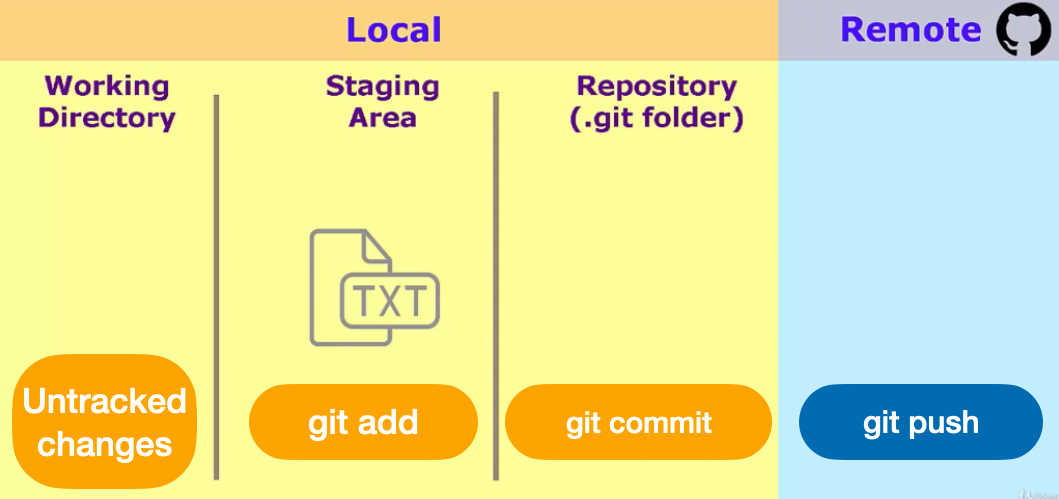
\includegraphics[width=0.5\textwidth]{images/git_stages.png}
				%				\vspace{-2mm}
				%				\captionof{figure}{Git states and associated commands. \href{https://www.udemy.com/course/git-complete/}{ \faLink{}  Source}}
				%			\end{minipage}
			
		\end{minipage}
	};
	\node[fancytitle, right=10pt, fill=outlinecolor, text=background, draw=outlinecolor, rounded corners] at (box.north west) {Tagging (2)};
\end{tikzpicture}